\chapter{ランサムウェア対策}
\section{感染リスクの緩和}
現実世界の攻撃を戦術と使用技術の観点から分類したフレームワークであるMITRE ATT\&CK \cite{MITREATT12:online}によると,
ランサムウェアのデータ侵害は,攻撃の最終段階であるImpactステージの
Data Destruction,
Data Encrypted for Impact,
Data Manipulation
のいずれかに分類される.
つまり,ランサムウェアによるデータ侵害はInitial Access (初期アクセス) や Privilege Escalation (権限昇格) などのステージを完了した後に発生するといえる.
したがって,Impactより前のステージにおけるセキュリティ強化もランサムウェア対策の重要な要素である.
なお,本研究の提案手法はランサムウェアのImpactステージの活動に対する対策であるため,本節の内容はスコープ外であることに注意する.
\begin{figure}[t]
  \begin{center}
    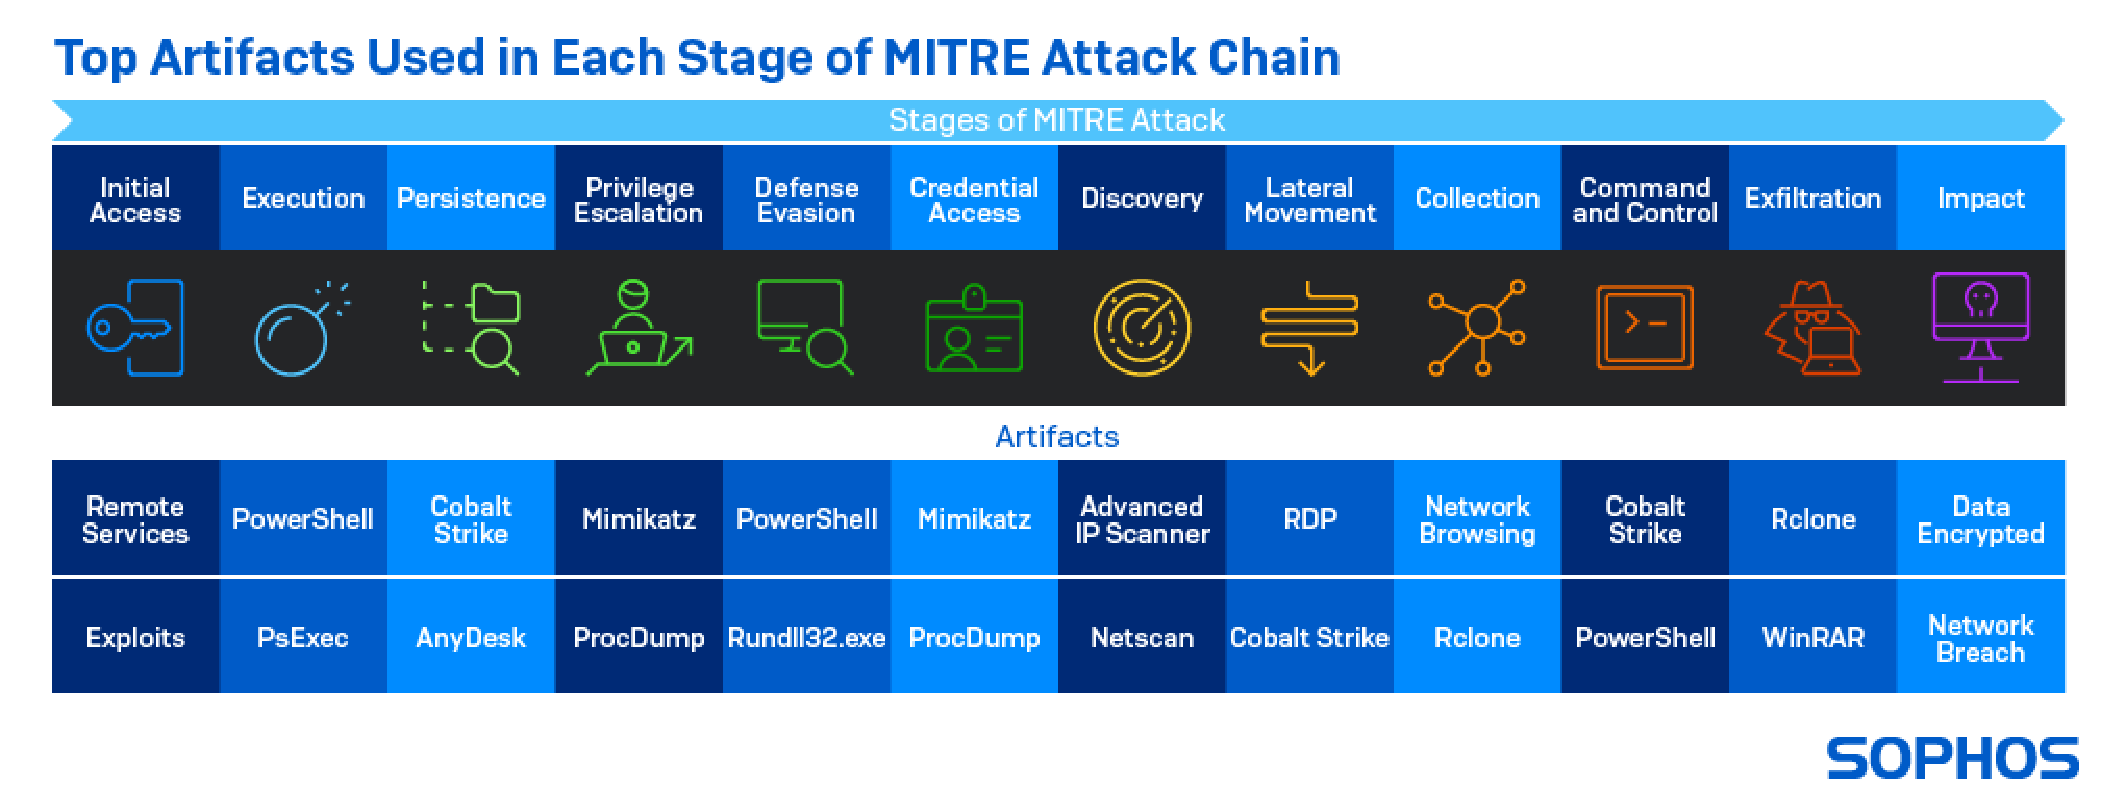
\includegraphics[width=0.8\columnwidth]{doc/img/mitre-attack-chain.eps}
  \end{center}
  \caption{Overview of each stage in MITRE ATT\&CK framework.
    Some stages such as Reconnaissance are omitted for simplicity. \cite{mitre-explained}}
  \label{fig:mitre-attack-chain}
\end{figure}

本節では,すべてのランサムウェアが通過するステージであるInitial Accessステージに焦点を当て,感染リスクの緩和について述べる.
SpyCloud社 \cite{spycloud-ransomware} によると,ランサムウェアのInitial Accessに利用される手法として2023年に最も多く報告されたものは
フィッシング,サードパーティアプリケーションのIAM設定の不備,cookie窃取によるセッションハイジャックであった.
これらの手法に対する一般的な対策を\tabref{tab:initial-access}に示す.
\begin{table}[t]
  \centering
  \label{tab:initial-access}
  \caption{Techniques for Initial Access and general countermeasures}
  \begin{tabular}{|c|c|}
    \hline
    \textbf{Initial Accessの手法} & \textbf{対策} \\
    \hline
    フィッシング                     &
    \begin{tabular}{c}
      メールフィルタリングを強化する \\
      組織構成員の教育を行う
    \end{tabular}
    \\
    % Email filteringUser awareness training,         \\
    \hline
    IAM設定の不備                   &
    \begin{tabular}{c}
      多要素認証を導入する
      % Email filtering \\ User awareness training
    \end{tabular}
    \\
    \hline
    Cookie窃取によるセッションハイジャック     &
    \begin{tabular}{c}
      Secure属性やHTTPOnly属性を強制する \\
      多要素認証を導入する
    \end{tabular}
    \\
    \hline
  \end{tabular}
\end{table}

\section{ランサムウェア検知}
\subsection{特徴量}
ランサムウェアを検知する手法で用いられる特徴量は,
実行ファイルの解析から得られる静的データと,実行ファイルを実行した際にプロセスの振る舞いから得られる動的データに分類される.
静的データを用いた検知を静的検知,動的データを用いた検知を動的検知と呼ぶ.
静的検知と動的検知は組み合わせて使用されることもあり,これをハイブリッド検知と呼ぶ.

静的検知では実行ファイルにおけるランサムウェア特有の構造的特徴を分析する.
典型的な静的データはファイルのハッシュ値,文字列,関数呼び出しなどである .
文字列としては"ransom"や"bitcoin"などのランサムノートに頻出する文字列や,
過去にランサムウェアが使用していたドメイン文字列やIPアドレスなどが確認される\cite{berrueta2019survey}.
また関数呼び出しについては,暗号化やファイルアクセスといった操作の有無を,ランサムウェアと良性アプリケーションの区別に使用することができる \cite{Evolution-Ransomware}.
しかし,静的データは一般に難読化や圧縮などの手法に弱く,さらに新種のランサムウェアに対して有効ではないことが多いという問題が指摘されている \cite{mitigation-modern}.

